\subsection{Sprints}

\subsubsection{Sprint \#1}

\begin{center}
	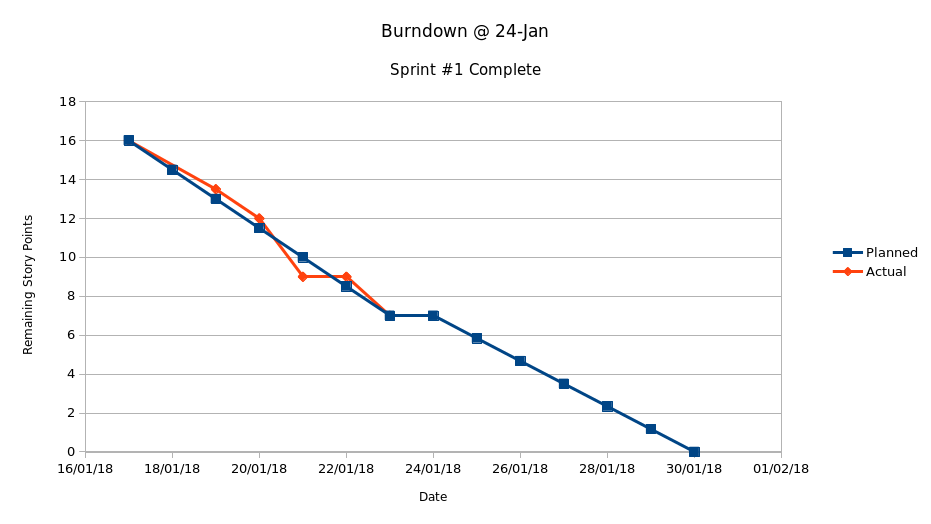
\includegraphics[scale=0.5]{burndown_1}
	\captionof{figure}{Burndown Chart Sprint \#1}
	\label{figure:burndown_1}
\end{center}

The upfront design work paid dividends during Sprint \#1, resulting in steady progress during implementation.
As noted in Appendix \ref{appendix:sprint2_planning_meeting}, some stories took longer than anticipated to complete, however the team stepped-up efforts to complete all stories within the iteration.

\subsubsection{Sprint \#2}

\begin{center}
	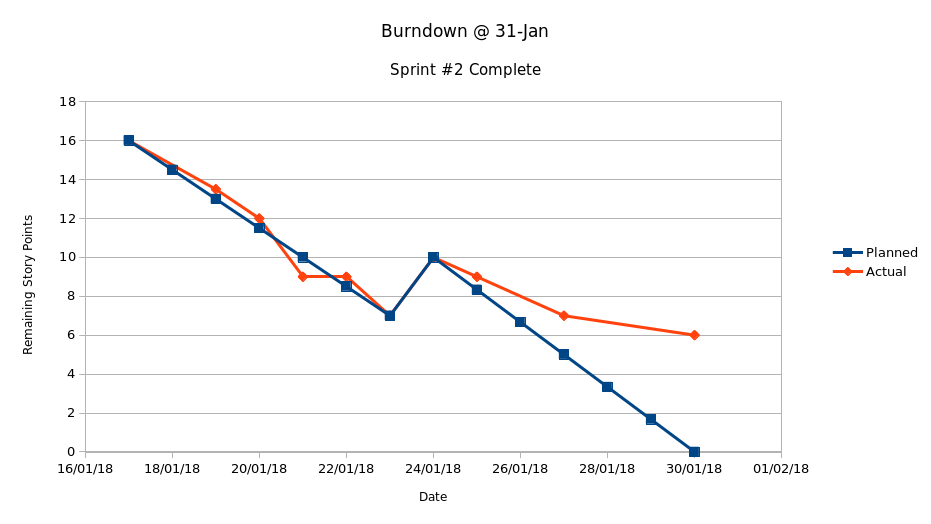
\includegraphics[scale=0.5]{burndown_2}
	\captionof{figure}{Burndown Chart Sprint \#2}
	\label{figure:burndown_2}
\end{center}

Sprint \#2 proved to be a challenge, due to the team's overall lack of experience with the online technologies, and the impact of some early decision decisions.
During Sprint \#1, the model (specifically the \texttt{Game} class, was implemented in a way that relied on a synchronous flow of events, with most game logic being contained in a single method. When the Observable \texttt{notify()} method was called at key stages to change \texttt{gameState}, execution was blocked, passing execution over to the controller where the event was handled. Upon completion of the controller flow, execution was handed back to the model where the logic continued.

However, due to the asyncronous, stateless nature of the online technologies, this blocking mechanism was no longer available.
The solution was to refactor the model to create individual methods for each segment of game logic, which would be triggered by the controller as needed.
The impact of this was that most stories could not be completed within the iteration, and a third sprint had to be scheduled.

Appendix \ref{appendix:sprint3_planning_meeting} has further details.

\subsubsection{Sprint \#3}

\begin{center}
	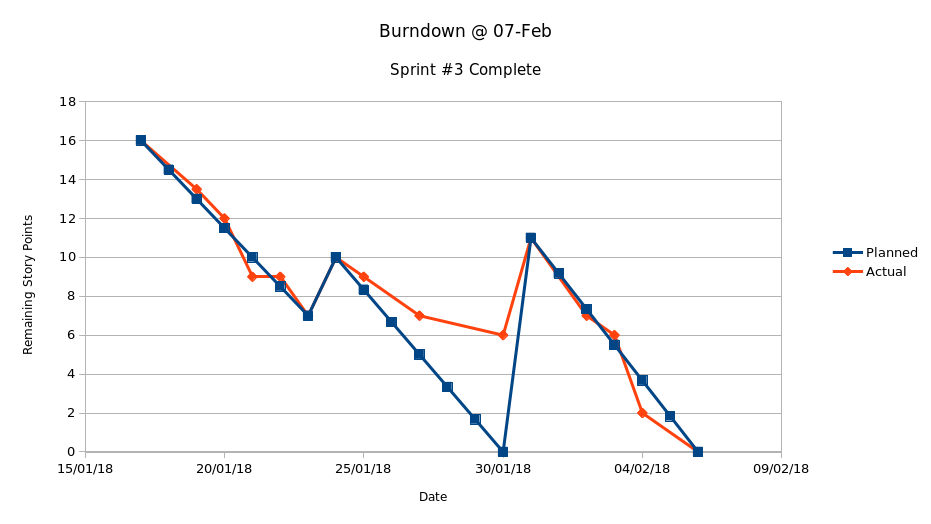
\includegraphics[scale=0.5]{burndown_3}
	\captionof{figure}{Burndown Chart Sprint \#3}
	\label{figure:burndown_3}
\end{center}

Sprint \#3 successfully solved the issues encountered previously, and the project came to a functional conclusion at the end of the iteration.

Appendix \ref{appendix:final_sprint_meeting} has further details.